\chapter{Klientska časť}
Táto časť poskytuje užívateľské rozhranie, naviguje užívateľa v~rámci aplikácie, reaguje na jeho akcie a komunikuje s~vystaveným rozhraním serverovej časti aplikácie.
\par Klienstka časť je naimplementovaná použitím frameworku Angular 2. Nejedná sa o~tzv. single page, ako je to bežné pri~aplikáciách napísaných v~tomto frameworku, ale je rozdelená na tri stránky, kde si každá drží svoj interný stav. Sú to stranký Miner, Mined Patterns a~Regex Groups. Stránka Miner slúži na samotné odhaľovanie parsovacích vzorov, zatiaľ čo Stránky Mined Patterns a Regex Groups slúžia na prácu s~finalizovanými parsovacími vzormi, resp. sadami typov regulárnych výrazov určených pre transformáciu vzorov.


\section{Angular 2}
Angular 2 je relatívne nový komponentovo-orientovaný JavaScriptový framework, ktorý odstraňuje nedostatky pôvodnej verzie. Aplikácie sa v~Angular 2 píšu buď v~TypeScripte, alebo vo verziách \mbox{ECMAScript}~5 resp. 6. Ani jeden variant zatiaľ nie je plne podporovaný dnešnými prehliadačmi, preto je nutná transkompilácia. My sme použili TypeScript, nadstavbu JavaScriptu, ktorý zavádza statické typovanie a~prvky objektovo-orientovaného programovania ako typy, triedy, moduly a~pod., čo považujeme za veľkú výhodu. Základné stavebné prvky sú:

\begin{enumerate}
 \item Modul -- zpuzdruje funkcionalitu, ktorá vykonáva jednu úlohu. Funguje podobne ako OSGi modul, kde modul vidí len komponenty definované v~samotnom module a komponenty, ktoré modul explicitne importuje. Zároveň modul špecifikuje, ktoré komponenty budú viditeľné zvonku balíčka.
 \item Komponent -- základný prvok aplikácie. Definuje aplikačnú logiku a interaguje so šablónou cez rozhranie vlastností a metód. Potrebná konfigurácia komponentu je zabezpečená cez metadáta.
 \item Šablóna -- html stránka obohatená o~značky z~jazyka Angular. Definuje, ako bude zobrazený komponent. Zároveň obsahuje značkovanie pre prepojenie dát, ktoré určuje, ako sú vymieňané dáta medzi komponentom a šablónou. V~predošlej verzii Angularu sa vždy jednalo o~obojsmerné prepojenie, čo spôsobovalo výkonnostné problémy. Vo verzii 2 si vieme toto prepojenie zašpecifikovať a vyhnúť sa tak týmto problémom.
 \item Servisná služba -- trieda, ktorá obsahuje funkcie na vykonanie špecifických úloh potrebných aplikáciou.
 \item Dependency injection -- spôsob založený na rovnomennom návr\-hovom vzore, ktorým Angular poskytuje servisným službám a~komponentom závislosti.
\end{enumerate}

\subsection{Podporné nástroje}
Aplikácie písané v~Angular 2 sú závislé na knižniciach tretích strán, ako aj na knižniciach samotného Angularu.
\par Na správu týchto závislostí používame všeobecne známy Node.js a~jeho balíčkovací systém npm, zatiaľ čo na správu samotného kódu používame Webpack, jednoduchý balíčkovač zdrojových kódov. Webpack ponúka široké možnosti ako zdrojové kódy upraviť pred výsledným zabalením do archívu, a zároveň možnosť vystaviť tieto kódy v~rámci vývojového servera, čo sme pri vývoji vo veľkej miere využívali. V~našom systéme Webpack pred výsledným zabalením zdrojové kódy minimalizuje a prevedie optimalizácie.
\par Oba tieto nástroje sme ovládali a nastavovali cez nástroj Angular CLI, ktorý umožnuje vygenerovať si projekt už obsahujúci najčastejšiu konfiguráciu.


\subsection{Miner}
Na začiatku je možné určiť aplikáciu, z~ktorej analyzované správy pochádzajú, a jej verziu, ako môžeme vidieť na obr. \ref{fig:miner-source}. Ďalej môžeme určiť, či chceme analyzovať správy z~logovacieho súboru, ktorý nahrajeme, alebo použijeme správy, ktoré už sú v~systéme nahrané a neboli zatiaľ finálne analyzované.

\begin{figure}[htbp]
 \centering 
 \begin{minipage}{0.95\linewidth}
 	\centering
 	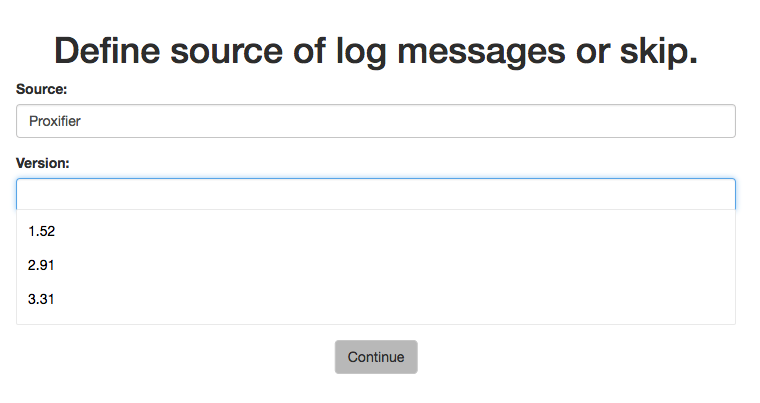
\includegraphics[width=\textwidth]{Images/thesis-miner-source.png}
 \end{minipage}
  \caption{Špecifikovanie zdrojovej aplikácie pre potreby analýzy. \mbox{Vstupné} polia sú umiestnené pod sebou, ako reakcia na šírku okna v~responzívnom dizajne.}
  \label{fig:miner-source}
\end{figure}

Po tomto kroku máme pred sebou rozhranie, ktorým budeme upravovať a spúšťať analýzu.
\par Po upresnení oddeľovačov a q-percentilu užívateľ spustí analýzu. Po obdržaní výsledkov je užívateľovi prezentovaná tabuľka, ktorej hlavnú časť tvoria navrhované parsovacie vzory. V~tabuľke napravo je~tlačidlo, ktorým užívateľ daný parsovací vzor potvrdí ako finálny. Pre~potreby spresňujúcej analýzy je pri každom vzore vľavo checkbox. Pri~označení ľubovoľného počtu navrhovaných vzorov a následnej analýze sú ako vstupné správy brané len tie, ktoré prislúchali k~označeným vzorom. Výsledky spresňujúcej analýzy sú vložené do~tabuľky tak, že novo navrhované parsovacie vzory sú pripojené ako potomkovia vzoru, z~ktorého vznikli, a vytvárajú tak stromovú štruktúru. Tento proces vieme opakovať, až kým nefinalizujeme všetky parsovacie vzory, alebo sa môžeme rozhodnúť pre začatie novej analýzy.

\begin{figure}[htbp]
 \centering 
 \begin{minipage}{0.95\linewidth}
 	\centering
 	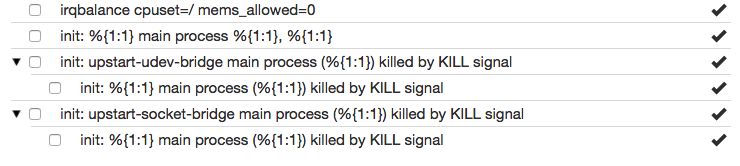
\includegraphics[width=\textwidth]{Images/thesis-miner-analysis.png}
 \end{minipage}
  \caption{Priebeh analýzy logovacích správ.}
  \label{fig:miner-source}
\end{figure}

\subsection{Mined patterns}
Rozhranie prezentuje stránkovací zoznam finalizovaných parsovacích vzorov, ktoré si je možné vyfiltrovať podľa zdrojovej aplikácie a jej verzie, ako vidíme na obrázku \ref{fig:pattern}. Aktuálny vyfiltrovaný zoznam si~užívateľ vie exportovať do formátu REtrie. Zoznam ďalej umožnuje náhľad na správy, ktoré boli vygenerované, použitím vybraného parsovacieho vzoru.

\begin{figure}[htbp]
 \centering 
 \begin{minipage}{0.95\linewidth}
 	\centering
 	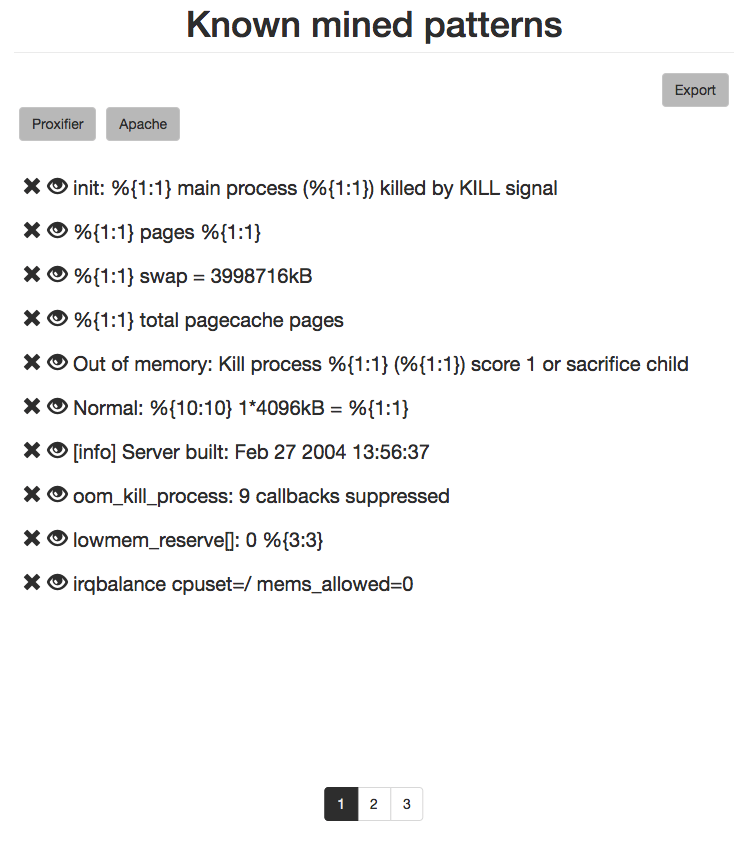
\includegraphics[width=\textwidth]{Images/thesis-pattern.png}
 \end{minipage}
  \caption{Správa uložených parsovacích vzorov.}
  \label{fig:pattern}
\end{figure}

\subsection{Regex Groups}
Zobrazuje zoznam sád typov regulárnych výrazov, ktoré sú v~aplikácií nahrané. V~systéme sme prednastavili základnú sadu, ktorá by mala byť postačujúca pre značnú časť prípadov a táto sada nejde zo systému zmazať. Systém ďalej umožnuje nahrať novú sadu zo súboru vo~formáte:

 \begin{figure}[htbp]
 \centering 
 \begin{minipage}{0.95\linewidth}
 	\centering
 	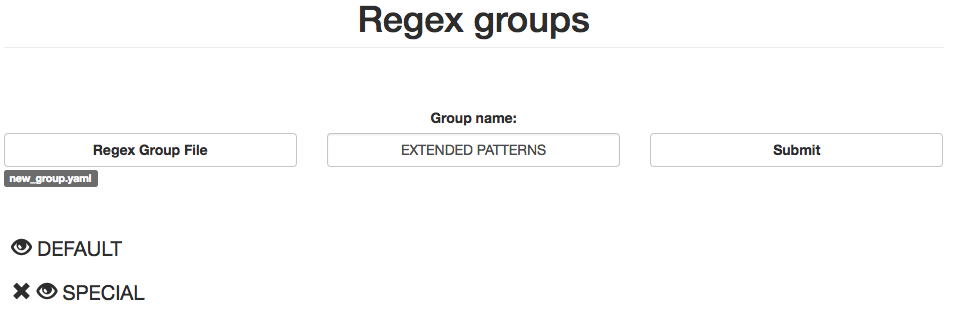
\includegraphics[width=\textwidth]{Images/thesis-groups.png}
 \end{minipage}
  \caption{Importovanie novej skupiny a aktuálny zoznam.}
  \label{fig:groups}
\end{figure}
